
\section{Clock Skew Sensitivity}
\label{sec:results:csmb_sensitivity}

Previous sections have explained how Sniper speeds up simulation compared to common cycle accurate simulators by utilizing one separate simulation thread per simulated core.
In order to correctly simulate inter-core interactions, the simulation threads need to be kept in sync.
The method used to keep the threads in sync affects both simulation accuracy and simulation time.
By having a relaxed synchronization method, one can improve simulation time, at the cost of simulation accuracy.
In our experiments, we have used barrier synchronization with a barrier width of 100 cycles.
This entails that for every 100 simulated cycles the separate threads synchronize.
Any inter-core interactions that occur between barriers are not guaranteed to happen in the correct order, but events from different barrier intervals will happen in the correct order.


\begin{figure}
    \centering
    \begin{subfigure}[b]{0.5\textwidth}
        \includegraphics[width=\textwidth]{figures/results/speedup/csmb-stp-0128k-0100-csmb-4}
        \caption{STP sensitivity to CSMB}
        \label{fig:results:base:csmb:stp}
    \end{subfigure}%
    \begin{subfigure}[b]{0.5\textwidth}
        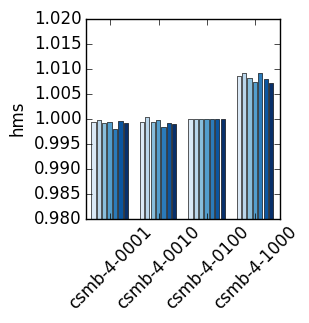
\includegraphics[width=\textwidth]{figures/results/speedup/csmb-hms-0128k-0100-csmb-4}
        \caption{HMS sensitivty to CSMB}
        \label{fig:results:base:csmb:hms}
    \end{subfigure}
    \begin{subfigure}[b]{0.6\textwidth}
        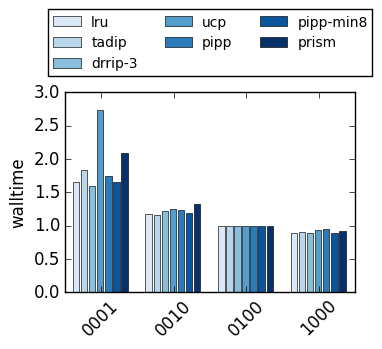
\includegraphics[width=\textwidth]{figures/results/speedup/csmb-walltime-0128k-0100-csmb-4}
        \caption{walltime sensitivity to CSMB}
        \label{fig:results:base:csmb:mpki}
    \end{subfigure}
    \caption{STP, HMS and walltime sensitivity to size of CSMB}
    \label{fig:results:csmb}
\end{figure}



We devised an experiment where we vary the value of the clock skew minimization barrier (CSMB) and compare average STP, HMS and mpki values for all 4-core workloads.
Figure~\ref{fig:results:csmb} contains plots for both STP and HMS relative to the default 100 cycle barrier.
From the graph, it is apparent that lowering the value below 100 cycles causes negligible variations in our average values. 
The most noticeable is PIPP, but it varies less than 0.2\% with a tighter barrier interval.
Increasing the interval to 1000 cycles results in a more noticeable difference in measurements.
For both HMS, shown in figure~\ref{fig:results:csmb:hms}, and mpki, not shown, the trends are the same.
Variance in simulation time relative to CSMB values, as shown in figure~\ref{fig:results:csmb:walltime} is as expected. 
When lowering the barrier interval we see an increase in average simulation time while increasing the interval gives a decrease.
We do note that the simulation time difference between the default value of 100 cycles and 1000 cycles is small.
This observation in combination with the variance observed in the other variables leads us to believe that 100 cycles are a good middle ground between performance and accuracy.

